
%***************************************************************************
%
% CreditCruncher - A portfolio credit risk valorator
% Copyright (C) 2004 Gerard Torrent
%
% This program is free software; you can redistribute it and/or
% modify it under the terms of the GNU General Public License
% as published by the Free Software Foundation; either version 2
% of the License.
%
% This program is distributed in the hope that it will be useful,
% but WITHOUT ANY WARRANTY; without even the implied warranty of
% MERCHANTABILITY or FITNESS FOR A PARTICULAR PURPOSE.  See the
% GNU General Public License for more details.
%
% You should have received a copy of the GNU General Public License
% along with this program; if not, write to the Free Software
% Foundation, Inc., 59 Temple Place - Suite 330, Boston, MA 02111-1307, USA.
%
%
% formulation.tex - TeX documentation file
% --------------------------------------------------------------------------
%
% 2005/01/22 - Gerard Torrent [gerard@fobos.generacio.com]
%   . initial release
%
%***************************************************************************

\chapter{Formulaci\'on del problema}
\label{sec:formulation}

Dada una cartera de cr\'editos a empresas de tama\~no mediano, deseamos 
valorar las posibles p\'erdidas debido a los impagos al cabo de un 
tiempo $T$.

En este cap\'itulo se introducen los elementos considerados claves para la 
definici\'on del problema.

TODO: No se considera clave la obtenci\'on de las matrices de correlaci\'on y 
transici\'on (v\'ease bibliograf\'ia).


%---------------------------------------------------------------------------

\section{Cartera de cr\'editos}

La estructura de la cartera de cr\'editos consiste en un conjunto de
clientes agrupados por sectores de actividad. Cada cliente tiene contratado 
un conjunto de productos de cr\'edito. Cada contrato puede estar 
cubierto por un n\'umero variable de garant\'ias o acuerdos.
Puede verse un esquema de la estructura en la figura \ref{portfolio}.

\begin{figure}[!hb]
\begin{center}
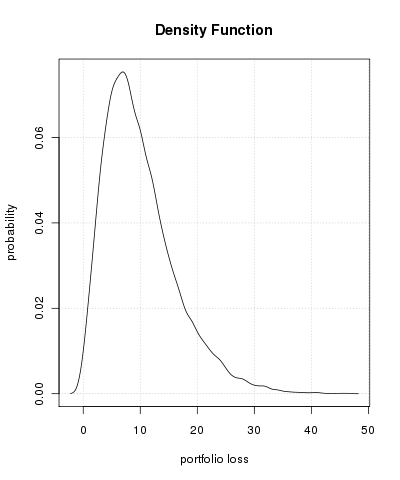
\includegraphics[angle=-90]{./images/portfolio.epsi}
\caption{Estructura de la cartera de cr\'editos}
\label{portfolio}
\end{center}
\end{figure}


\subsection{Ratings}

\begin{figure}[!hb]
\begin{center}
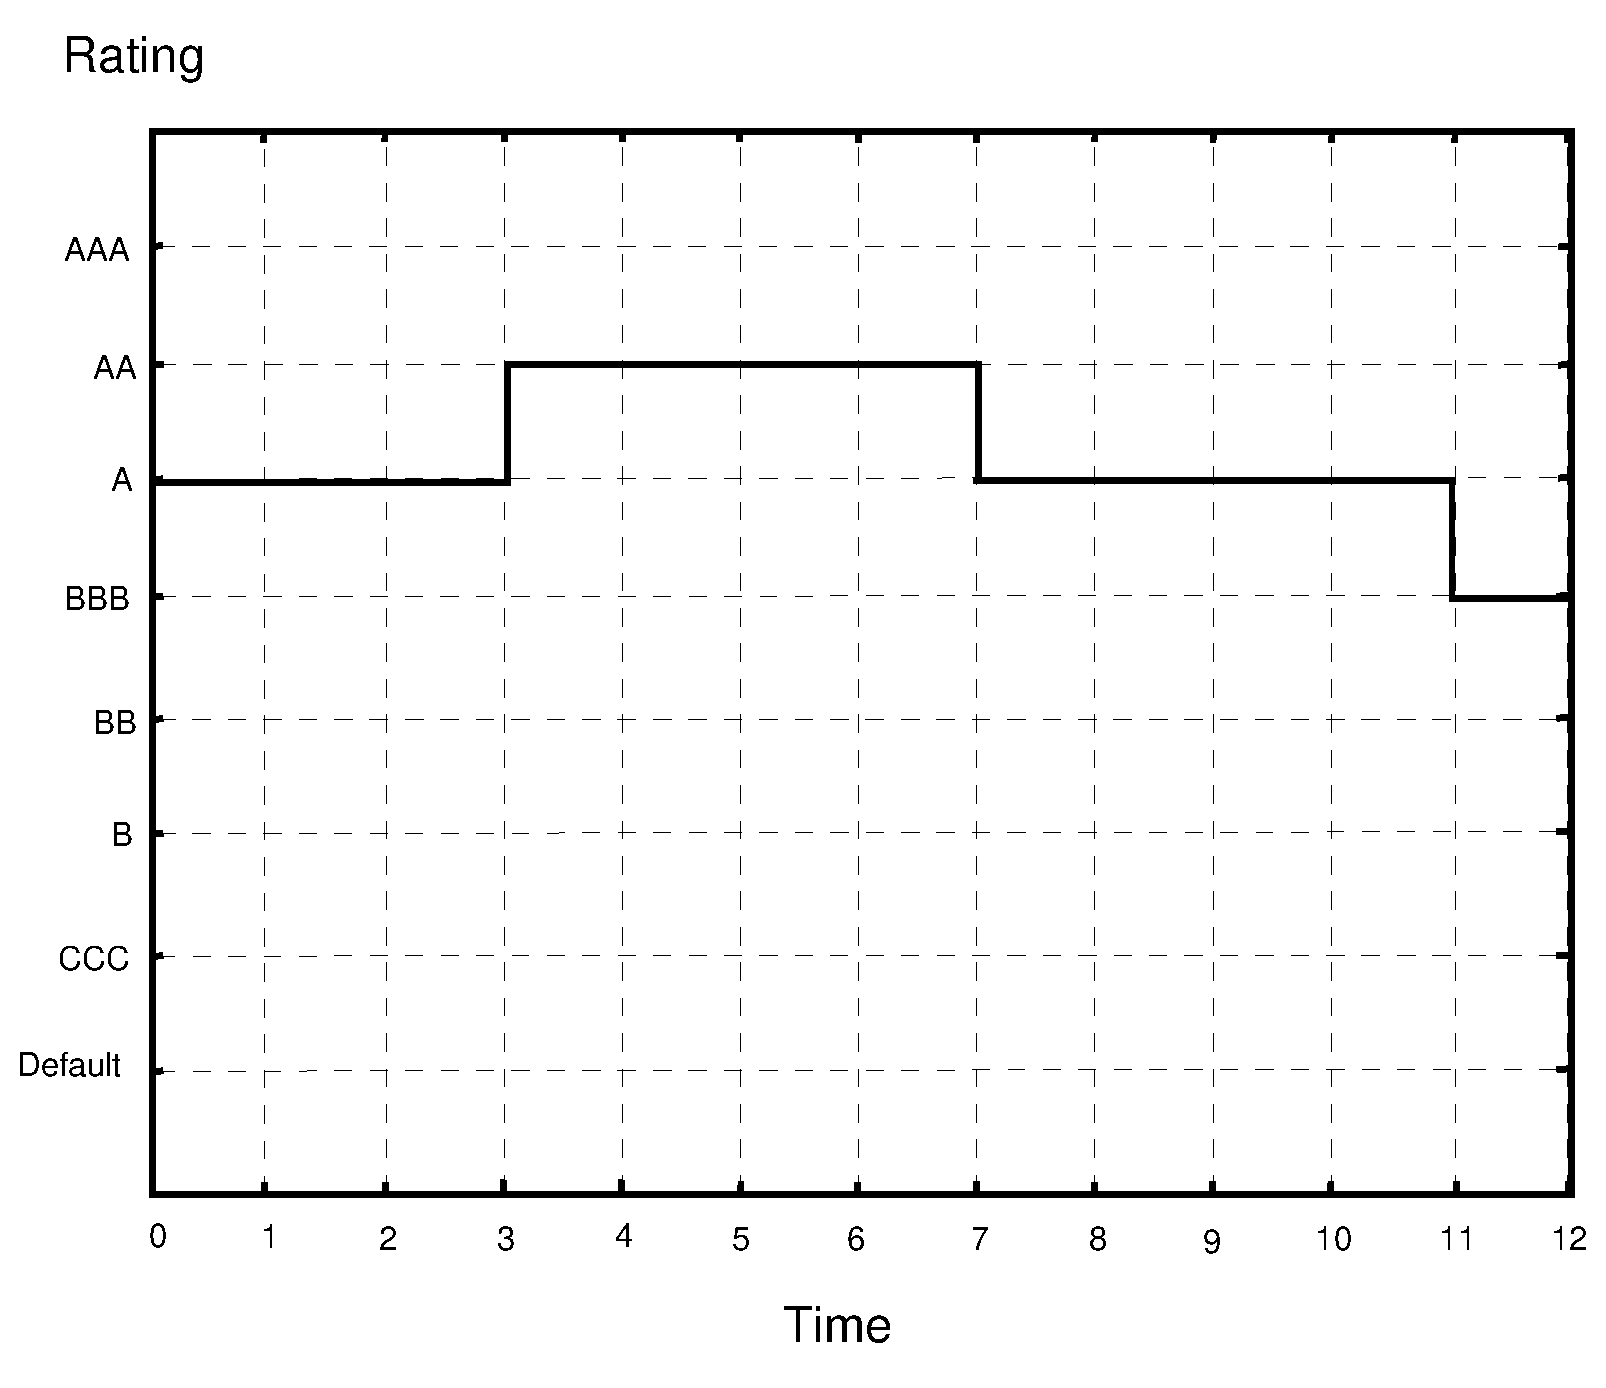
\includegraphics[height=7cm, angle=0]{./images/ratingevol.eps}
\caption{Evoluci\'on del rating a lo largo del tiempo}
\label{ratingevol}
\end{center}
\end{figure}

\subsection{Productos}

\subsection{Sectores}

\subsection{Exposici\'on}

\subsection{Severidad}

%---------------------------------------------------------------------------

\section{Value At Risk (VAR)}

\begin{figure}[!hb]
\begin{center}
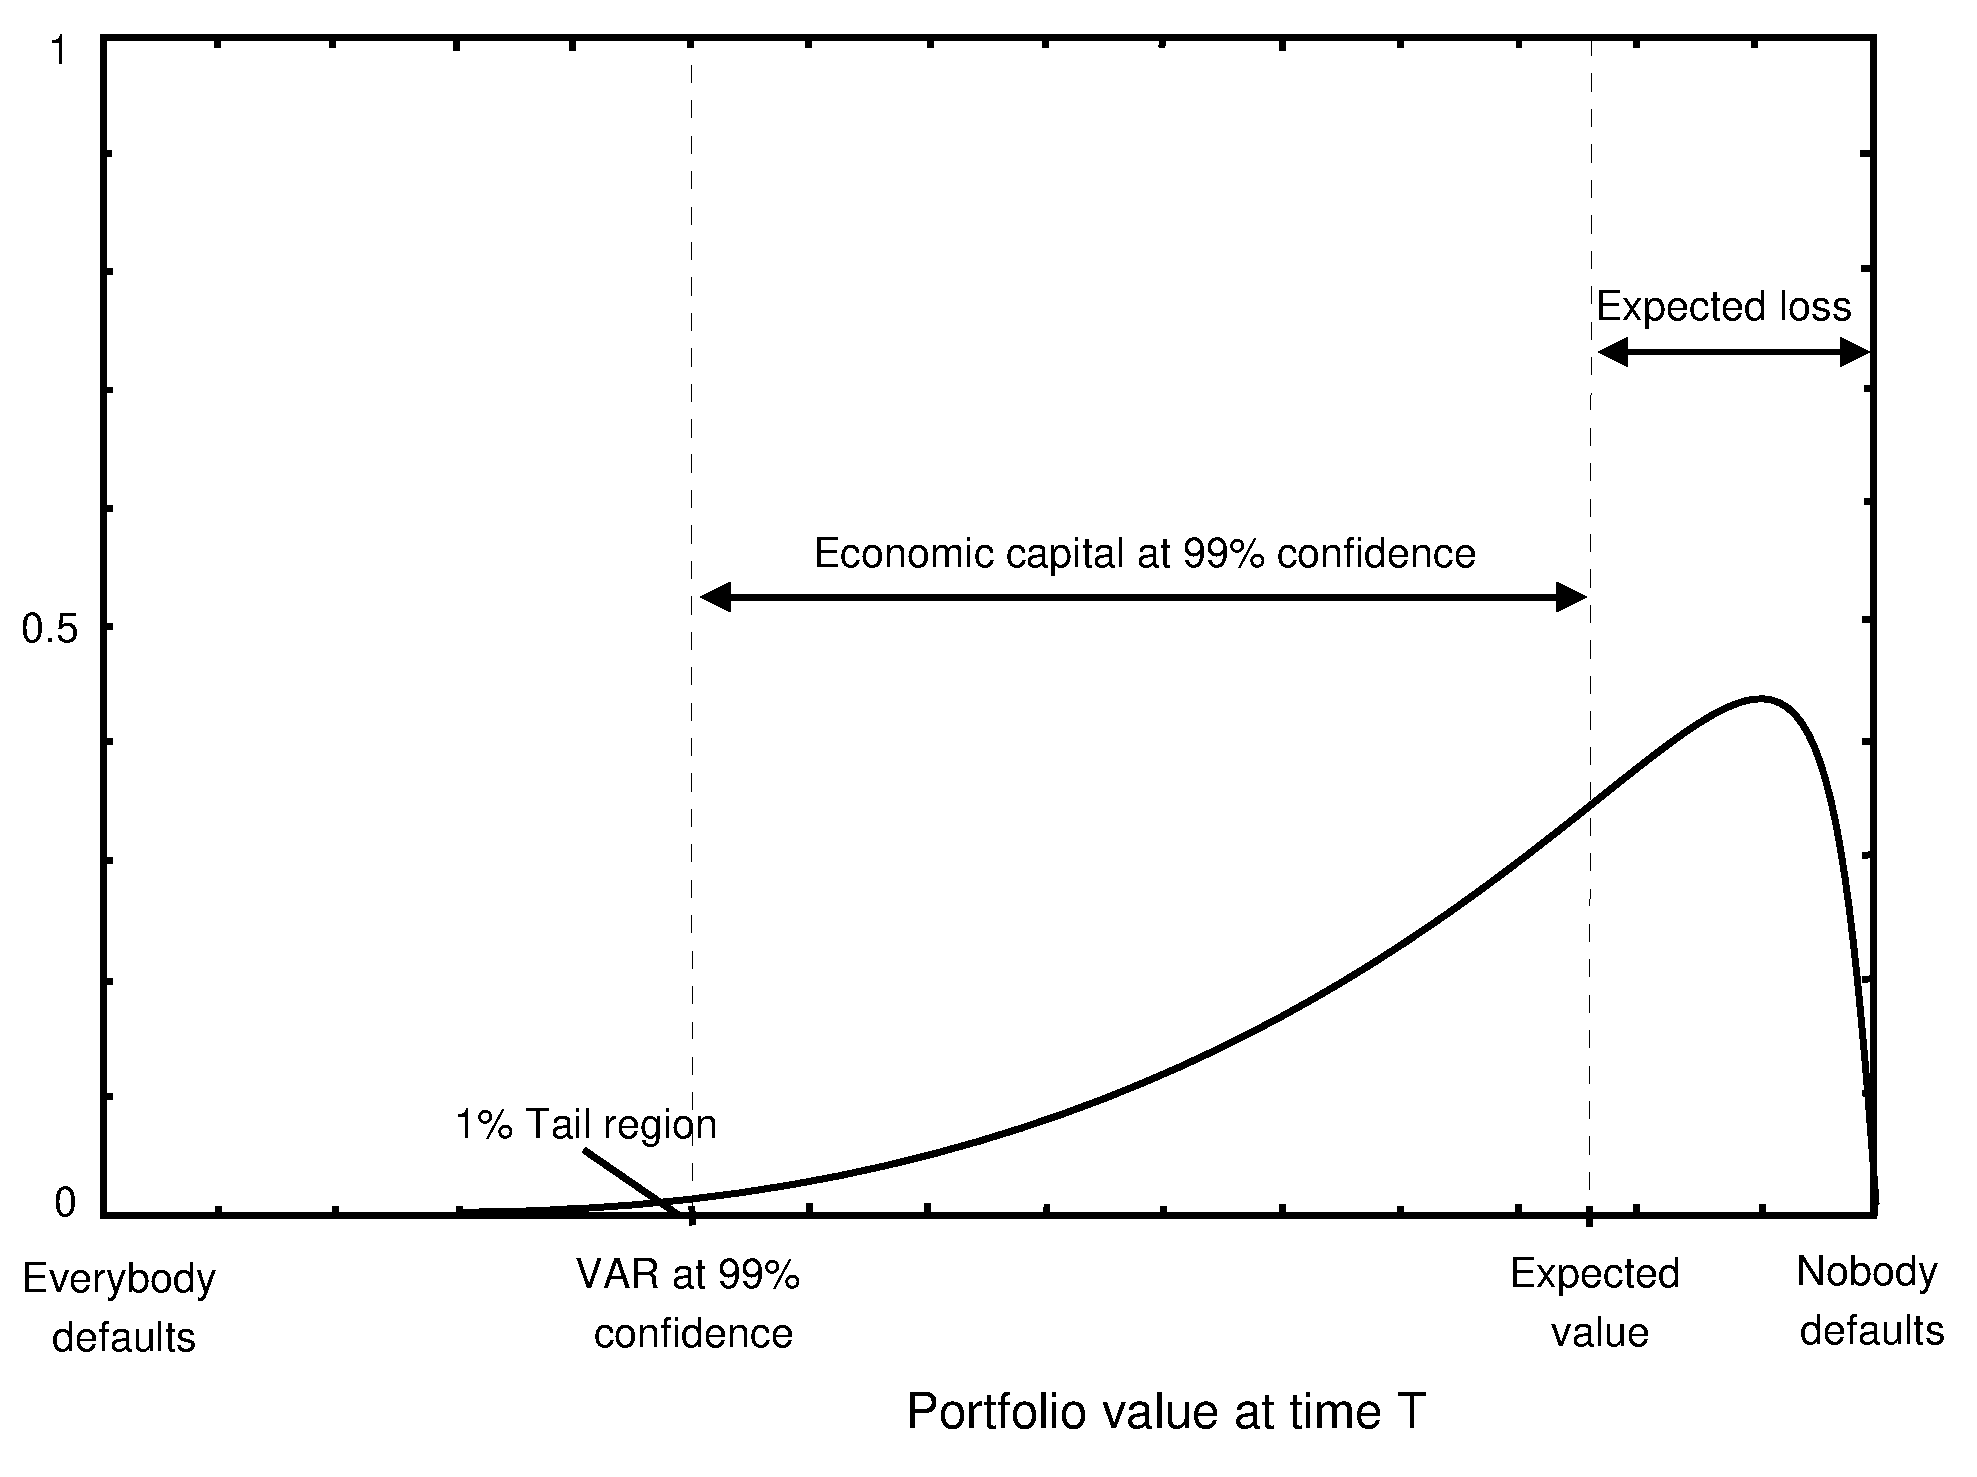
\includegraphics[height=7cm, angle=0]{./images/creditvar.eps}
\caption{Distribuci\'on del valor de la cartera y c\'alculo del VAR}
\label{creditvar}
\end{center}
\end{figure}

%---------------------------------------------------------------------------

\section{Matriz de transici\'on}

\subsection{Definici\'on.} La matriz de transici\'on nos proporciona la probabilidad 
que un cliente con rating inicial $r_i$ pase a tener, al cabo de un tiempo $T$, 
rating $r_j$. La denotamos de la forma siguiente:

\begin{displaymath}
M_T = \left(
\begin{array}{ccc}
m_{1,1} & \dots  & m_{1,n} \cr
\vdots & \ddots & \vdots \cr
m_{n,1} & \dots  & m_{n,n} 
\end{array}
\right)
\end{displaymath}

\noindent donde cada elemento de la matrix, $m_{i,j}$ corresponde a la 
probabilidad de que un cliente con rating $r_i$ pase a tener, al cabo de $T$ 
tiempo, rating $r_j$.

\subsection{Ejemplo.} Matriz de transici\'on anual ($T=1$ a\~no) extraida del 
documento \emph{CreditMetrics. Technical Document}. Las probabilidades est\'an
expresadas en tanto por ciento.
\\
\begin{center}
\begin{tabular}[]{l|rrrrrrrr}
        &      AAA &       AA &        A &      BBB &       BB &        B &      CCC &  Default \cr
\hline
AAA     &  $90.81$ &   $8.33$ &   $0.68$ &   $0.06$ &   $0.12$ &   $0.00$ &   $0.00$ &   $0.00$ \cr
 AA     &   $0.70$ &  $90.65$ &   $7.79$ &   $0.64$ &   $0.06$ &   $0.14$ &   $0.02$ &   $0.00$ \cr
  A     &   $0.09$ &   $2.27$ &  $91.05$ &   $5.52$ &   $0.74$ &   $0.26$ &   $0.01$ &   $0.06$ \cr
BBB     &   $0.02$ &   $0.33$ &   $5.95$ &  $86.93$ &   $5.30$ &   $1.17$ &   $0.12$ &   $0.18$ \cr
 BB     &   $0.03$ &   $0.14$ &   $0.67$ &   $7.73$ &  $80.53$ &   $8.84$ &   $1.00$ &   $1.06$ \cr
  B     &   $0.00$ &   $0.11$ &   $0.24$ &   $0.43$ &   $6.48$ &  $83.46$ &   $4.07$ &   $5.20$ \cr
CCC     &   $0.22$ &   $0.00$ &   $0.22$ &   $1.30$ &   $2.38$ &  $11.24$ &  $64.86$ &  $19.79$ \cr
Default &   $0.00$ &   $0.00$ &   $0.00$ &   $0.00$ &   $0.00$ &   $0.00$ &   $0.00$ & $100.00$
\end{tabular}
\end{center}
\noindent en particular, la probabilidad que un cliente con rating $AA$ pase a 
tener rating $B$ al cabo de un a\~no es del $0.14\%$.

\subsection{Propiedades}

\paragraph{Propiedad 1.}
El valor de los elementos de la matriz de transici\'on se encuentran entre $0$ 
y $1$ debido a que son probabilidades.

\begin{displaymath}
0 \leq m_{i,j} \leq 1 \quad \forall i,j
\end{displaymath}

\paragraph{Propiedad 2.}
La suma de los elementos de cualquier fila de la matriz de transici\'on suman $1$.
De esta forma se  est\'a imponiendo que el conjunto de ratings finales solo puede 
ser el de los ratings contemplados en la matriz.

\begin{displaymath}
\sum_{j=1}^{n} m_{i,j} = 1 \quad \forall i
\end{displaymath}

\paragraph{Propiedad 3.}
Los elementos de la fila correspondiente al rating $default$, son todos $0$,
excepto el elemento de la columna que corresponde al rating $default$ que vale 
$1$. Esta condici\'on indica que cuando se llega al estado de fallido no es 
posible salir de este estado.

\begin{displaymath}
\begin{array}{ll}
m_{default,j} = 0        & \quad \forall j \neq default \cr
m_{default,default} = 1
\end{array}
\end{displaymath}


\subsection{Cambio de periodo}

Deseamos obtener la matriz de transici\'on para periodos distintos (m\'ultiplos o 
fraccionarios) del periodo proporcionado, $T$. Esto nos permitir\'a determinar la 
probabilidad que un cliente con rating inicial $r_i$ tenga rating $r_j$ al cabo 
de $x \cdot T$ tiempo.

\paragraph{Ejemplo.} Calculemos la probabilidad de pasar de rating $AA$ a
rating $B$ en un plazo de dos a\~nos disponiendo de la matriz de transici\'on anual.

\begin{displaymath}
\begin{array}{llll}
P(AA \to B;2) = & P(AA \to AAA;1)    & \cdot P(AAA \to B;1)      & + \cr
                & P(AA \to AA;1)      & \cdot P(AA \to B;1)      & + \cr
                & P(AA \to A;1)       & \cdot P(A \to B;1)       & + \cr
                & P(AA \to BBB;1)     & \cdot P(BBB \to B;1)     & + \cr
                & P(AA \to BB;1)      & \cdot P(BB \to B;1)      & + \cr
                & P(AA \to B;1)       & \cdot P(B \to B;1)       & + \cr
                & P(AA \to CCC;1)     & \cdot P(CCC \to B;1)     & + \cr
                & P(AA \to default;1) & \cdot P(default \to B;1) &
\end{array}
\end{displaymath}

\paragraph{Proposici\'on} Sean $M_{T_1}$ y $M_{T_2}$ las matrices de transici\'on
para los periodos $T_1$ y $T_2$. Entonces, la matriz de transici\'on para el
periodo $T_1+T_2$ es:
\begin{displaymath}
M_{T_1+T_2} = M_{T_1} \cdot M_{T_2}
\end{displaymath}

\paragraph{Corolario} Sean $M_{T}$ la matriz de transici\'on para el periodo 
$T$ y $k \in \mathrm{N}$. Entonces:
\begin{displaymath}
M_{k \cdot T} = M_{T}^k
\end{displaymath}
\begin{displaymath}
M_{\frac{T}{k}} = \sqrt[k]{M_{T}}
\end{displaymath}


\subsection{Tasa de morosidad anticipada}


%---------------------------------------------------------------------------

\section{Matriz de correlaci\'on sectorial}


